\documentclass[12pt,a4paper]{article}

\usepackage[margin=1in]{geometry}
\usepackage{pgfgantt}
\usepackage{amssymb}
\usepackage{tikz}
\usetikzlibrary{arrows.meta, positioning, shapes.geometric, calc}
\usepackage{booktabs}
\usepackage{hyperref}
\usepackage{enumitem}
\usepackage{titlesec}
\usepackage{fancyhdr}
\usepackage{xcolor}
\usepackage{array}
\usepackage{tabularx}

% ── Colours ───────────────────────────────────────────────
\definecolor{phaseA}{HTML}{4A90D9}
\definecolor{phaseB}{HTML}{50C878}
\definecolor{phaseC}{HTML}{FF8C42}
\definecolor{phaseD}{HTML}{E8665D}
\definecolor{phaseE}{HTML}{9B59B6}
\definecolor{critical}{HTML}{E74C3C}
\definecolor{noncrit}{HTML}{3498DB}
\definecolor{headblue}{HTML}{1A5276}

\titleformat{\section}
  {\Large\bfseries\color{headblue}}
  {\thesection.}{0.5em}{}[\vspace{2pt}\titlerule]
\titleformat{\subsection}
  {\large\bfseries\color{headblue!80}}
  {\thesubsection}{0.5em}{}

\pagestyle{fancy}
\setlength{\headheight}{14.5pt}
\addtolength{\topmargin}{-2.5pt}
\fancyhf{}
\lhead{\small\textit{Project Plan --- CA Firm System}}
\rhead{\small\textit{Group E-17}}
\cfoot{\thepage}

\begin{document}

% ═══════════════════════════════════════════════════════════
\begin{titlepage}
\centering
\vspace*{2cm}
{\Huge\bfseries\color{headblue} Software Project Plan\\[12pt]}
{\LARGE CA Firm Attendance and\\Article Management System\\[20pt]}
\rule{0.6\textwidth}{1pt}\\[20pt]

{\large\textbf{Assignment No. 7}}\\[30pt]

\begin{tabular}{ll}
\textbf{Group:} & E-17 \\[4pt]
\textbf{Members:} & Nivesh Jain \\
 & Harsh Nayak \\
 & Rachit Ingole \\
 & Hasan Rupawalla \\
\end{tabular}

\vfill
{\small Department of Computer Engineering\\
\today}
\end{titlepage}

% ═══════════════════════════════════════════════════════════
\section{Problem Statement}
% ═══════════════════════════════════════════════════════════
Prepare a detailed software project plan for the development of a \textbf{CA Firm Attendance and Article Management System}. The project plan should incorporate scheduling techniques such as Gantt charts and PERT charts to map out the development timeline, visualize task dependencies, and determine the critical path of the project.

% ═══════════════════════════════════════════════════════════
\section{Abstract}
% ═══════════════════════════════════════════════════════════
Effective project planning forms the backbone of any successful software development endeavor. It encompasses task identification, effort estimation, dependency mapping, and continuous progress tracking. This document presents a comprehensive project plan for the \textbf{CA Firm Attendance and Article Management System} --- a web-based platform that automates attendance tracking (biometric face recognition + GPS), task assignment, leave management, and performance reporting for a Chartered Accountant firm. The plan employs a Work Breakdown Structure (WBS), a Gantt chart for timeline visualization, and a PERT chart for dependency and critical path analysis.

% ═══════════════════════════════════════════════════════════
\section{Introduction}
% ═══════════════════════════════════════════════════════════
Modern software systems demand rigorous planning to navigate the complexities of multi-module architectures, third-party integrations, and iterative feedback cycles. A well-defined project plan mitigates risks such as schedule overruns, scope creep, and inefficient resource allocation.

The \textbf{CA Firm Attendance and Article Management System} is developed for SPCM (CA Firm) to replace paper-based article trainee management. It integrates biometric face recognition (face-api.js), GPS-based geofencing (Browser Geolocation API), task assignment with progress tracking, leave management, and analytics dashboards (Chart.js). The system is built on React.js, Node.js/Express, and MySQL.

\subsection{Planning Objectives}
\begin{enumerate}[noitemsep, label=\roman*)]
    \item Decompose the project into well-defined, manageable tasks.
    \item Estimate realistic durations for each development activity.
    \item Map inter-task dependencies to identify sequencing constraints.
    \item Construct a visual project schedule with specific calendar dates.
    \item Highlight the critical path to focus monitoring efforts.
    \item Anticipate risks and establish mitigation strategies.
\end{enumerate}

% ═══════════════════════════════════════════════════════════
\section{Development Phases}
% ═══════════════════════════════════════════════════════════
The project timeline spans from \textbf{January 19, 2026} to \textbf{April 28, 2026} (approximately 14 weeks). The lifecycle is divided into eight phases:

\begin{center}
\begin{tabular}{cl}
\toprule
\textbf{\#} & \textbf{Phase} \\
\midrule
1 & Requirement Analysis \& SRS \\
2 & System \& Architecture Design \\
3 & Database Schema Design (MySQL) \\
4 & Backend Development (Node.js/Express) \\
5 & Frontend Development (React.js) \\
6 & Face Recognition \& GPS Integration \\
7 & Testing \& Quality Assurance \\
8 & Deployment \& Documentation \\
\bottomrule
\end{tabular}
\end{center}

% ═══════════════════════════════════════════════════════════
\section{Work Breakdown Structure}
% ═══════════════════════════════════════════════════════════
The WBS decomposes the project into discrete tasks with estimated durations, specific calendar dates, and explicit dependency chains.

\bigskip
\begin{center}
\small
\begin{tabularx}{\textwidth}{c X c c c}
\toprule
\textbf{ID} & \textbf{Task} & \textbf{Duration} & \textbf{Start Date} & \textbf{End Date} \\
\midrule
T1 & Requirement Analysis \& SRS & 2 Weeks & 19 Jan 2026 & 01 Feb 2026 \\
T2 & System \& Architecture Design & 1.5 Weeks & 02 Feb 2026 & 12 Feb 2026 \\
T3 & Database Schema Design & 1.5 Weeks & 02 Feb 2026 & 12 Feb 2026 \\
T4 & Backend: Auth, CRUD, Task APIs & 3 Weeks & 13 Feb 2026 & 05 Mar 2026 \\
T5 & Backend: Attendance \& Leave APIs & 2 Weeks & 06 Mar 2026 & 19 Mar 2026 \\
T6 & Frontend: Core Pages \& Dashboard & 3 Weeks & 13 Feb 2026 & 05 Mar 2026 \\
T7 & Frontend: Attendance \& Reports UI & 2 Weeks & 06 Mar 2026 & 19 Mar 2026 \\
T8 & Face Recognition + GPS Integration & 2 Weeks & 20 Mar 2026 & 02 Apr 2026 \\
T9 & Testing \& QA & 2 Weeks & 03 Apr 2026 & 16 Apr 2026 \\
T10 & Deployment \& Documentation & 1.5 Weeks & 17 Apr 2026 & 28 Apr 2026 \\
\bottomrule
\end{tabularx}
\end{center}

\subsection{Task Descriptions}

\textbf{T1 --- Requirement Analysis \& SRS (Jan 19 -- Feb 1):}
Stakeholder interviews with SPCM (CA firm), feature prioritization, and preparation of the IEEE 830 SRS document. Core requirements include biometric attendance, task management, leave management, and reporting.

\textbf{T2 --- System \& Architecture Design (Feb 2 -- Feb 12):}
Defines the three-tier architecture: React.js SPA (frontend), Node.js/Express REST API (backend), MySQL database (data layer), and Python face recognition microservice. Includes API endpoint design and component interaction diagrams.

\textbf{T3 --- Database Schema Design (Feb 2 -- Feb 12):}
Creates 9 MySQL tables: admins, articles (with face\_descriptor), attendance, tasks, task\_assignments, progress\_log, leave\_requests, notifications, and settings. Establishes foreign key relationships and indexes.

\textbf{T4 --- Backend: Auth, CRUD, Task APIs (Feb 13 -- Mar 5):}
Implements JWT authentication with bcrypt hashing, role-based access control (Admin/Article), article trainee CRUD operations, task creation/assignment APIs, and progress tracking endpoints.

\textbf{T5 --- Backend: Attendance \& Leave APIs (Mar 6 -- Mar 19):}
Develops the attendance recording API (face descriptor comparison + GPS coordinate validation using Haversine formula), geofencing logic (configurable 100m radius), leave request/approval workflow, and notification triggers via Nodemailer.

\textbf{T6 --- Frontend: Core Pages \& Dashboard (Feb 13 -- Mar 5):}
Builds the React.js SPA with login page, admin dashboard (overview metrics), article management page, task management page, and responsive navigation. Runs in parallel with T4.

\textbf{T7 --- Frontend: Attendance \& Reports UI (Mar 6 -- Mar 19):}
Develops the attendance marking page (camera feed + GPS indicator), attendance history view, leave application form, analytics dashboard with Chart.js visualizations, and report export (PDF/CSV). Runs in parallel with T5.

\textbf{T8 --- Face Recognition + GPS Integration (Mar 20 -- Apr 2):}
Integrates face-api.js for browser-based face detection and descriptor matching, implements camera MediaDevices API access, connects Geolocation API for GPS coordinates, and links frontend attendance flow with backend verification.

\textbf{T9 --- Testing \& QA (Apr 3 -- Apr 16):}
Unit tests for API endpoints, integration tests for attendance flow (face + GPS + database), leave workflow testing, report generation validation, and UAT with SPCM stakeholders.

\textbf{T10 --- Deployment \& Documentation (Apr 17 -- Apr 28):}
Deploy backend on Render/AWS, frontend on Vercel. Finalize blackbook documentation, user manual, and project handover to SPCM.

% ═══════════════════════════════════════════════════════════
\section{Project Scheduling}
% ═══════════════════════════════════════════════════════════

\subsection{Gantt Chart}
The Gantt chart maps each task against the 14-week calendar timeline (Jan 19 -- Apr 28, 2026), with color-coded bars and dependency arrows.

\bigskip
\begin{center}
\resizebox{\textwidth}{!}{%
\begin{ganttchart}[
    hgrid,
    vgrid={*{6}{draw=gray!25}, *1{draw=gray!60}},
    x unit=0.17cm,
    y unit chart=0.65cm,
    title height=1,
    title label font=\tiny\bfseries,
    bar label font=\scriptsize,
    bar height=0.6,
    link/.style={->, thick, gray!70},
    time slot format=isodate
]{2026-01-19}{2026-04-28}

  \gantttitlecalendar{year, month=shortname} \\

  \ganttbar[bar/.append style={fill=phaseA}, name=t1]{T1: Requirement Analysis \& SRS}{2026-01-19}{2026-02-01} \\
  \ganttbar[bar/.append style={fill=phaseA}, name=t2]{T2: System Design}{2026-02-02}{2026-02-12} \\
  \ganttbar[bar/.append style={fill=phaseB}, name=t3]{T3: Database Schema Design}{2026-02-02}{2026-02-12} \\
  \ganttbar[bar/.append style={fill=phaseC}, name=t4]{T4: Backend: Auth + CRUD + Tasks}{2026-02-13}{2026-03-05} \\
  \ganttbar[bar/.append style={fill=phaseC}, name=t5]{T5: Backend: Attendance + Leave}{2026-03-06}{2026-03-19} \\
  \ganttbar[bar/.append style={fill=phaseC}, name=t6]{T6: Frontend: Core + Dashboard}{2026-02-13}{2026-03-05} \\
  \ganttbar[bar/.append style={fill=phaseC}, name=t7]{T7: Frontend: Attendance + Reports}{2026-03-06}{2026-03-19} \\
  \ganttbar[bar/.append style={fill=phaseD!80!black}, name=t8]{T8: Face Recog. + GPS Integration}{2026-03-20}{2026-04-02} \\
  \ganttbar[bar/.append style={fill=phaseD}, name=t9]{T9: Testing \& QA}{2026-04-03}{2026-04-16} \\
  \ganttbar[bar/.append style={fill=phaseE}, name=t10]{T10: Deployment \& Docs}{2026-04-17}{2026-04-28} \\

  % Dependencies
  \ganttlink{t1}{t2}
  \ganttlink{t1}{t3}
  \ganttlink{t2}{t4}
  \ganttlink{t3}{t4}
  \ganttlink{t2}{t6}
  \ganttlink{t4}{t5}
  \ganttlink{t6}{t7}
  \ganttlink{t5}{t8}
  \ganttlink{t7}{t8}
  \ganttlink{t8}{t9}
  \ganttlink{t9}{t10}

\end{ganttchart}
}% end resizebox
\end{center}

\medskip
\noindent\textbf{Legend:}
\textcolor{phaseA}{$\blacksquare$}~Planning/Design \quad
\textcolor{phaseB}{$\blacksquare$}~Database \quad
\textcolor{phaseC}{$\blacksquare$}~Development \quad
\textcolor{phaseD}{$\blacksquare$}~Integration/Testing \quad
\textcolor{phaseE}{$\blacksquare$}~Deployment

\begin{center}
\small\textit{Figure 1: Gantt Chart --- CA Firm System (Jan 19 -- Apr 28, 2026)}
\end{center}

\subsection{Gantt Chart Analysis}
The timeline reveals several optimization strategies:
\begin{itemize}[noitemsep]
    \item \textbf{Parallel Design:} T2 (System Design) and T3 (Database Schema) execute concurrently during Feb 2--12, saving 1.5 weeks.
    \item \textbf{Parallel Development:} T4 (Backend core) and T6 (Frontend core) run simultaneously during Feb 13 -- Mar 5, leveraging the 4-member team.
    \item \textbf{Parallel Modules:} T5 (Backend attendance/leave) and T7 (Frontend attendance/reports) overlap during Mar 6--19.
    \item \textbf{Integration Gate:} T8 (Face Recognition + GPS) begins only after both backend and frontend attendance modules are complete (Mar 20).
    \item \textbf{Buffer:} 1.5 weeks of deployment time includes documentation slack.
\end{itemize}

% ─────────────────────────────────────────────────────────
\subsection{PERT Chart}
The PERT diagram represents tasks as nodes with directed edges indicating dependencies. The \textcolor{critical}{\textbf{critical path}} is highlighted in red.

\bigskip
\begin{center}
\resizebox{\textwidth}{!}{%
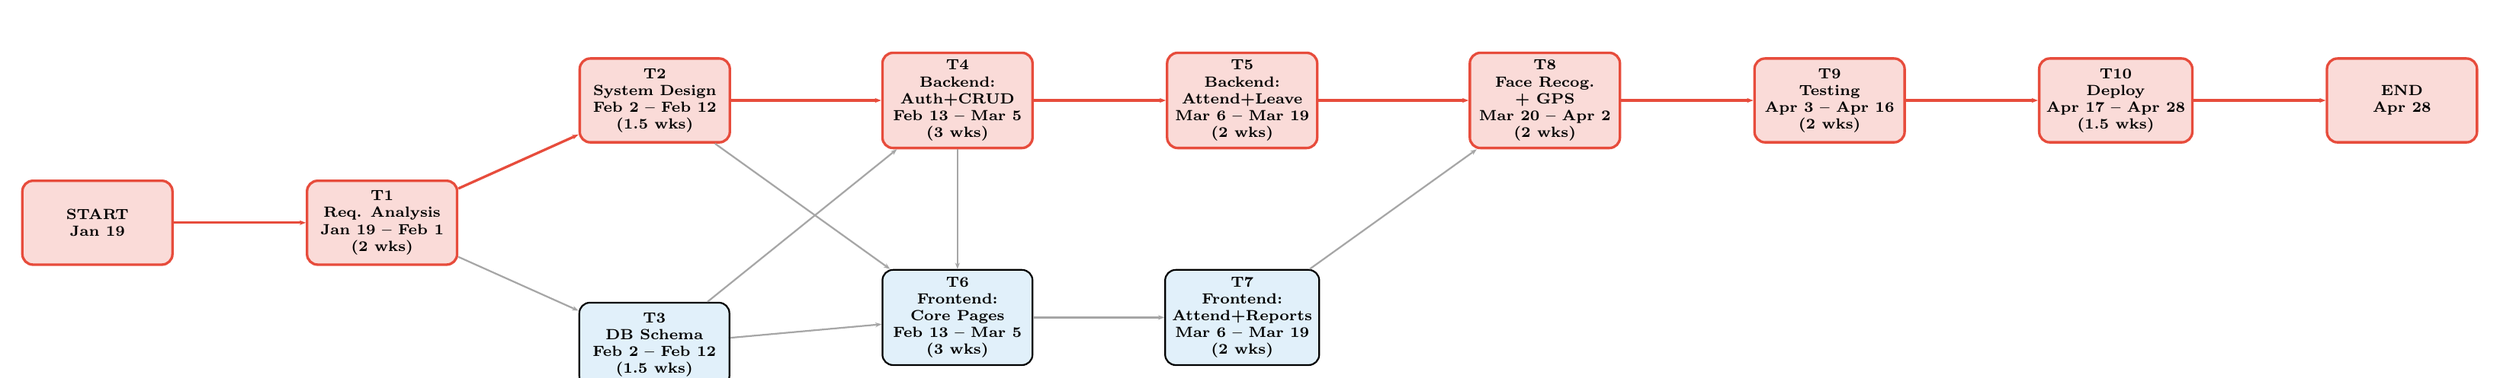
\begin{tikzpicture}[
    node distance=1.4cm and 2.2cm,
    task/.style={
        rectangle, rounded corners=5pt, draw, thick,
        minimum width=2.5cm, minimum height=1.4cm,
        align=center, font=\scriptsize\bfseries,
        fill=noncrit!15, text=black
    },
    crit/.style={
        task, fill=critical!20, draw=critical, very thick
    },
    arr/.style={-{Stealth[length=3pt]}, thick, gray!70},
    critarr/.style={-{Stealth[length=3pt]}, very thick, critical},
]

% ── Row 1 ────────────────────────────
\node[crit] (start) {START\\Jan 19};
\node[crit, right=of start] (T1) {T1\\Req. Analysis\\Jan 19 -- Feb 1\\(2 wks)};
\node[crit, above right=0.6cm and 2cm of T1] (T2) {T2\\System Design\\Feb 2 -- Feb 12\\(1.5 wks)};
\node[task, below right=0.6cm and 2cm of T1] (T3) {T3\\DB Schema\\Feb 2 -- Feb 12\\(1.5 wks)};

% ── Row 2 ────────────────────────────
\node[crit, right=2.5cm of T2] (T4) {T4\\Backend:\\Auth+CRUD\\Feb 13 -- Mar 5\\(3 wks)};
\node[task, below=2cm of T4] (T6) {T6\\Frontend:\\Core Pages\\Feb 13 -- Mar 5\\(3 wks)};

% ── Row 3 ────────────────────────────
\node[crit, right=of T4] (T5) {T5\\Backend:\\Attend+Leave\\Mar 6 -- Mar 19\\(2 wks)};
\node[task, below=2cm of T5] (T7) {T7\\Frontend:\\Attend+Reports\\Mar 6 -- Mar 19\\(2 wks)};

% ── Row 4 ────────────────────────────
\node[crit, right=2.5cm of T5] (T8) {T8\\Face Recog.\\+ GPS\\Mar 20 -- Apr 2\\(2 wks)};
\node[crit, right=of T8] (T9) {T9\\Testing\\Apr 3 -- Apr 16\\(2 wks)};
\node[crit, right=of T9] (T10) {T10\\Deploy\\Apr 17 -- Apr 28\\(1.5 wks)};
\node[crit, right=of T10] (finish) {END\\Apr 28};

% ── Critical Path (Red) ──────
\draw[critarr] (start) -- (T1);
\draw[critarr] (T1) -- (T2);
\draw[critarr] (T2) -- (T4);
\draw[critarr] (T4) -- (T5);
\draw[critarr] (T5) -- (T8);
\draw[critarr] (T8) -- (T9);
\draw[critarr] (T9) -- (T10);
\draw[critarr] (T10) -- (finish);

% ── Non-Critical (Gray) ──────
\draw[arr] (T1) -- (T3);
\draw[arr] (T3) -- (T4);
\draw[arr] (T2) -- (T6);
\draw[arr] (T3) -- (T6);
\draw[arr] (T4) -- (T6);
\draw[arr] (T6) -- (T7);
\draw[arr] (T7) -- (T8);

\end{tikzpicture}
}% end resizebox
\end{center}

\begin{center}
\small\textit{Figure 2: PERT Chart --- Task Dependencies and Critical Path}
\end{center}

\subsection{Critical Path Identification}
The critical path comprises the longest chain of dependent tasks:

\begin{center}
\textcolor{critical}{\textbf{T1 $\rightarrow$ T2 $\rightarrow$ T4 $\rightarrow$ T5 $\rightarrow$ T8 $\rightarrow$ T9 $\rightarrow$ T10}}
\end{center}

\begin{center}
\begin{tabular}{llccc}
\toprule
\textbf{Task} & \textbf{Dates} & \textbf{Duration} & \textbf{Cumulative} & \textbf{Critical?} \\
\midrule
T1: Requirement Analysis & Jan 19 -- Feb 1 & 2.0 wks & 2.0 wks & \textcolor{critical}{\textbf{Yes}} \\
T2: System Design & Feb 2 -- Feb 12 & 1.5 wks & 3.5 wks & \textcolor{critical}{\textbf{Yes}} \\
T3: Database Schema & Feb 2 -- Feb 12 & 1.5 wks & 3.5 wks & No (parallel) \\
T4: Backend Auth+CRUD & Feb 13 -- Mar 5 & 3.0 wks & 6.5 wks & \textcolor{critical}{\textbf{Yes}} \\
T5: Backend Attend+Leave & Mar 6 -- Mar 19 & 2.0 wks & 8.5 wks & \textcolor{critical}{\textbf{Yes}} \\
T6: Frontend Core & Feb 13 -- Mar 5 & 3.0 wks & --- & No (parallel) \\
T7: Frontend Attend+Rpts & Mar 6 -- Mar 19 & 2.0 wks & --- & No (parallel) \\
T8: Face Recog. + GPS & Mar 20 -- Apr 2 & 2.0 wks & 10.5 wks & \textcolor{critical}{\textbf{Yes}} \\
T9: Testing \& QA & Apr 3 -- Apr 16 & 2.0 wks & 12.5 wks & \textcolor{critical}{\textbf{Yes}} \\
T10: Deployment & Apr 17 -- Apr 28 & 1.5 wks & \textbf{14.0 wks} & \textcolor{critical}{\textbf{Yes}} \\
\bottomrule
\end{tabular}
\end{center}

\noindent\textbf{Total Critical Path Duration:} $2.0 + 1.5 + 3.0 + 2.0 + 2.0 + 2.0 + 1.5 = \mathbf{14.0~weeks}$ (Jan 19 -- Apr 28, 2026)

\medskip
\noindent Non-critical tasks T3, T6, and T7 carry approximately \textbf{1--2 weeks of float}, meaning minor delays in frontend or database design will not impact the overall schedule.

% ═══════════════════════════════════════════════════════════
\section{Risk Assessment}
% ═══════════════════════════════════════════════════════════

\begin{center}
\begin{tabularx}{\textwidth}{l X l}
\toprule
\textbf{Risk} & \textbf{Description} & \textbf{Mitigation} \\
\midrule
Face Recog. & face-api.js accuracy may drop in low-light or different angles & Confidence threshold 0.6 + re-capture prompt \\[4pt]
GPS Accuracy & Indoor GPS may drift beyond 100m geofence radius & Allow configurable radius + manual override by Admin \\[4pt]
Camera Access & Browser may deny camera/GPS permissions (HTTPS required) & HTTPS-only deployment + user permission guide \\[4pt]
Data Security & Biometric face descriptors are sensitive personal data & Encrypt at rest + do not store raw face images \\[4pt]
MySQL Perf. & Complex joins on attendance/task tables under concurrent load & Proper indexing + query optimization \\[4pt]
Team Avail. & Academic commitments may reduce bandwidth & Parallel tasks leverage 4-member team \\
\bottomrule
\end{tabularx}
\end{center}

% ═══════════════════════════════════════════════════════════
\section{Conclusion}
% ═══════════════════════════════════════════════════════════
This document presented a structured project plan for the CA Firm Attendance and Article Management System spanning January 19 to April 28, 2026. The Work Breakdown Structure decomposed the project into ten manageable tasks with specific calendar dates. The Gantt chart provided a visual timeline showing parallel development workstreams across the four-member team, and the PERT chart identified a 14-week critical path through the project lifecycle.

By leveraging these project management techniques, the development team can track progress against specific milestones, identify schedule risks early through critical path monitoring, and deliver the system to SPCM within the planned 14-week window.

\end{document}
